\subsection{The specular family retains the nonzero kinematic branch}

The nonzero kinematic branch is treated separately because the $00L$ rod passes through the reciprocal origin. For one crystallite orientation, write the rod as
\begin{equation}
  \vect{Q}(u)=u\unitvect{d}.
\end{equation}
The elastic condition is
\begin{equation}
  |\vect{k}_i+u\unitvect{d}|^2=|\vect{k}_i|^2.
\end{equation}
Expanding the left-hand side gives
\begin{equation}
  u\left(2\vect{k}_i\!\cdot\!\unitvect{d}+u\right)=0.
\end{equation}
The first solution, $u=0$, is the direct-beam point $\vect{Q}=0$. The second solution is the nonzero kinematic $00L$ branch,
\begin{equation}
  u^{\rm kin}_{00}=-2\vect{k}_i\!\cdot\!\unitvect{d}.
\end{equation}
If the rod direction is represented by a non-unit vector $\vect{d}$, the same derivation gives
\begin{equation}
  u^{\rm kin}_{00}=-2\frac{\vect{k}_i\!\cdot\!\vect{d}}{\vect{d}\!\cdot\!\vect{d}}.
\end{equation}
This derivation explains why the nonzero solution is used: the $u=0$ root identifies the direct beam, while the second root is the kinematic scattering point on the $00L$ rod.

\begin{figure}[H]
  \centering
  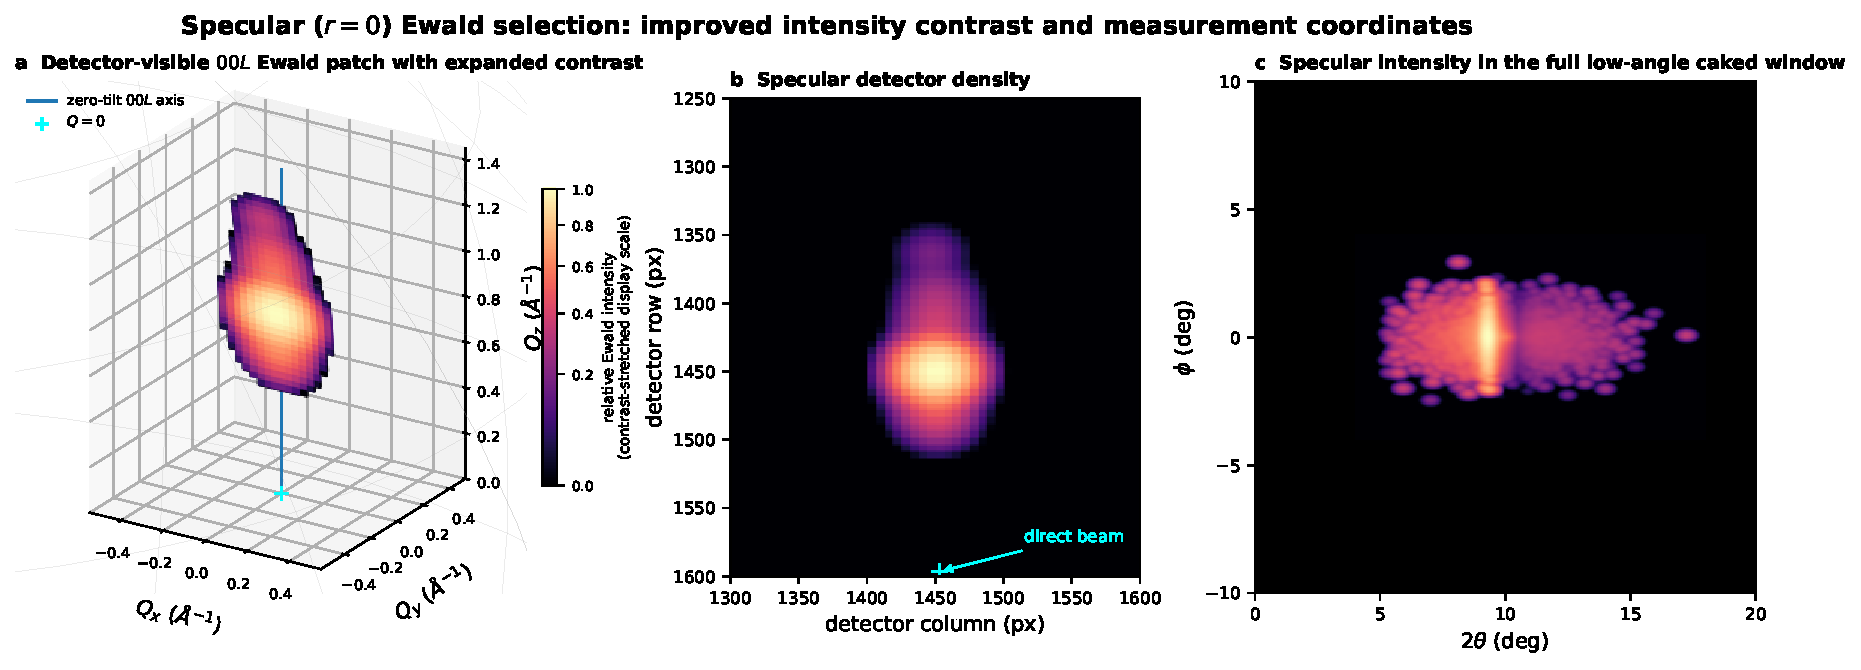
\includegraphics[width=\linewidth]{figures/fig_specular_detector_visible_round16.pdf}
  \caption{Specular ($r=0$) Ewald selection for the nominal Bi$_2$Se$_3$ incidence angle of $5^{\circ}$. (a) A local view centered on the detector-visible $00L$ Ewald patch, with the zero-tilt $00L$ axis and direct-beam point $\vect Q=0$ retained for reference. The color scale is reconstructed from the rendered detector field and contrast-stretched over its populated range so that the internal intensity variation across the patch is visible; it is a relative display scale rather than an additional physical normalization. (b) The corresponding specular detector density; the cyan cross marks the direct-beam coordinate. (c) The same specular intensity in the caked representation over the wider low-angle window $0^{\circ}\leq2\theta\leq20^{\circ}$ and $-10^{\circ}\leq\phi\leq10^{\circ}$. The calculated feature occupies the central part of this displayed angular region.}
\end{figure}
